\begin{flushright} {\tiny {\color{gray} volume\_hexahedron.tex}} \end{flushright}

What follows is based on the report "Efficient Computation of Volume of
Hexahedral Cells" by J. Grandy (1997) \cite{gran97}.
We assume the following internal numbering of the hexahedron,
which is different than the one in the paper: 

\begin{center}
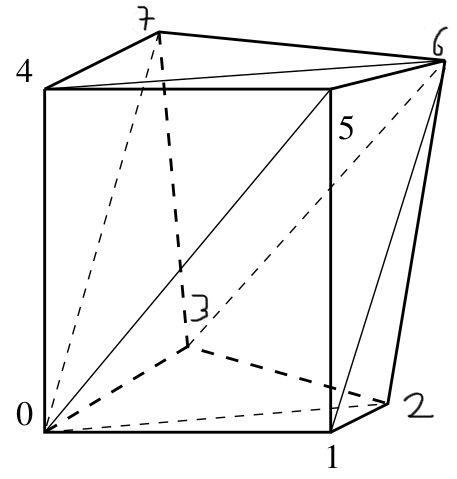
\includegraphics[width=3.4cm]{images/hexahedron/gran97}\\
{\captionfont Modified from \cite{gran97}}\\
{\tiny {\color{gray} in ./images/hexahedron/}}
\end{center}

If the hexahedron is such that some or all the opposite faces are planes parallel to 
each other than the volume can be arrived at very 
simply\footnote{\url{https://en.wikipedia.org/wiki/Cuboid}}.

The real catch here is that the four nodes which make up a face are not 
necessarily co-planar!  

The volume is then computed as follows
\begin{eqnarray}
V &=& [(\vec{r}_6-\vec{r}_1)+(\vec{r}_7-\vec{r}_0),(\vec{r}_6-\vec{r}_3),(\vec{r}_2-\vec{r}_0)] \nn\\
  &+& [(\vec{r}_7-\vec{r}_0),(\vec{r}_6-\vec{r}_3)+(\vec{r}_5-\vec{r}_0),(\vec{r}_6-\vec{r}_4)] \nn\\
  &+& [(\vec{r}_6-\vec{r}_1),(\vec{r}_5-\vec{r}_0),(\vec{r}_6-\vec{r}_4)+(\vec{r}_2-\vec{r}_0)] \nn\\
  &/& 12
\end{eqnarray}
where $[\cdot]$ is the triple product:
\[
[\vec{A},\vec{B},\vec{C}] = 
\left|
\begin{array}{ccc}
A_x & B_x & C_x \\
A_y & B_y & C_y \\
A_z & B_z & C_z 
\end{array}
\right|
\]
It is implemented and used in Stone 98. The code is shown hereunder:
\begin{lstlisting}
def hexahedron_volume (x,y,z):
    val = (  triple_product ( x[6]-x[1]+x[7]-x[0], y[6]-y[1]+y[7]-y[0], z[6]-z[1]+z[7]-z[0], \
                              x[6]-x[3],           y[6]-y[3],           z[6]-z[3],           \
                              x[2]-x[0],           y[2]-y[0],           z[2]-z[0]           )\
           + triple_product ( x[7]-x[0],           y[7]-y[0],           z[7]-z[0],           \
                              x[6]-x[3]+x[5]-x[0], y[6]-y[3]+y[5]-y[0], z[6]-z[3]+z[5]-z[0], \
                              x[6]-x[4],           y[6]-y[4],           z[6]-z[4]           )\
           + triple_product ( x[6]-x[1],           y[6]-y[1],           z[6]-z[1],           \
                              x[5]-x[0],           y[5]-y[0],           z[5]-z[0],           \
                              x[6]-x[4]+x[2]-x[0], y[6]-y[4]+y[2]-y[0], z[6]-z[4]+z[2]-z[0]  ) )/12.
    return val
\end{lstlisting}
with 
\begin{lstlisting}
def triple_product (Ax,Ay,Az,Bx,By,Bz,Cx,Cy,Cz):
    val = Ax * ( By * Cz - Bz * Cy )\
        - Ay * ( Bx * Cz - Bz * Cx )\
        + Az * ( Bx * Cy - By * Cx )
    return val
\end{lstlisting}

